\appendix

\chapter{Nodos desenvolvidos em Neo4J}

%\begin{appendices}

\section{Paciente}\label{secPaciente}
\begin{figure}[H]
    \centering
    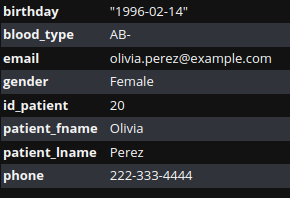
\includegraphics[width=0.3\linewidth]{Imagens/Neo4j/patient.png}
    \caption{Exemplo de um nodo paciente}
    \label{fig:nodo_paciente}
\end{figure}

\section{Seguro de Saúde}\label{secSeguroSaude}
\begin{figure}[H]
    \centering
    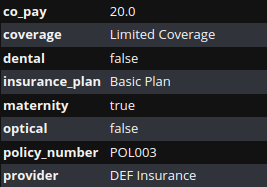
\includegraphics[width=0.3\linewidth]{Imagens/Neo4j/insurance.png}
    \caption{Exemplo de um nodo seguro de saúde}
    \label{fig:nodo_seguro_saude}
\end{figure}

\section{Histórico médico}\label{secHistoricoMedico}
\begin{figure}[H]
    \centering
    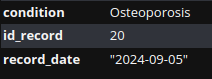
\includegraphics[width=0.3\linewidth]{Imagens/Neo4j/medical_history.png}
    \caption{Exemplo de um nodo histórico médico}
    \label{fig:nodo_historico_medico}
\end{figure}

\section{Contactos de Emergência}\label{secContactosEmergencia}
\begin{figure}[H]
    \centering
    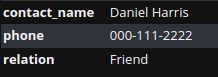
\includegraphics[width=0.3\linewidth]{Imagens/Neo4j/emergency_contact.png}
    \caption{Exemplo de um nodo contactos de emergência}
    \label{fig:nodo_contactos_emergencia}
\end{figure}

\section{Episódios Médicos}\label{secEpisodiosMedicos}
\begin{figure}[H]
    \centering
    
\includegraphics[width=0.3\linewidth]{Imagens/Neo4j/episode.png}
    \caption{Exemplo de um nodo episódios médicos}
    \label{fig:nodo_episodios_medicos}
\end{figure}

\section{Faturas}\label{secFaturas}
\begin{figure}[H]
    \centering
    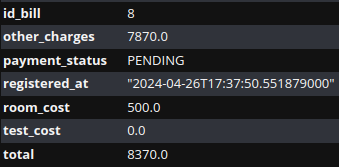
\includegraphics[width=0.3\linewidth]{Imagens/Neo4j/bill.png}
    \caption{Exemplo de um nodo faturas}
    \label{fig:nodo_faturas}
\end{figure}

\section{Prescrição Médica}\label{secPrescricaoMedica}
\begin{figure}[H]
    \centering
    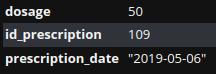
\includegraphics[width=0.3\linewidth]{Imagens/Neo4j/prescription.png}
    \caption{Exemplo de um nodo prescrição médica}
    \label{fig:nodo_prescricao_medica}
\end{figure}

\section{Medicamento}\label{secMedicamento}
\begin{figure}[H]
    \centering
    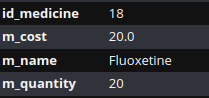
\includegraphics[width=0.3\linewidth]{Imagens/Neo4j/medicine.png}
    \caption{Exemplo de um nodo medicamento}
    \label{fig:nodo_medicamento}
\end{figure}

\section{Departamento}\label{secDepartamento}
\begin{figure}[H]
    \centering
    
\includegraphics[width=0.3\linewidth]{Imagens/Neo4j/department.png}
    \caption{Exemplo de um nodo departamento}
    \label{fig:nodo_departamento}
\end{figure}

\section{Funcionários}\label{secFuncionarios}
\begin{figure}[H]
    \centering
    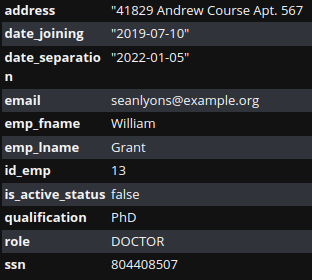
\includegraphics[width=0.3\linewidth]{Imagens/Neo4j/staff.png}
    \caption{Exemplo de um nodo funcionários}
    \label{fig:nodo_funcionarios}
\end{figure}

\section{Consulta}\label{secConsulta}
\begin{figure}[H]
    \centering
    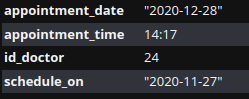
\includegraphics[width=0.3\linewidth]{Imagens/Neo4j/appointment.png}
    \caption{Exemplo de um nodo consulta}
    \label{fig:nodo_consulta}
\end{figure}

\section{Testes Médicos}\label{secTestesMedicos}
\begin{figure}[H]
    \centering
    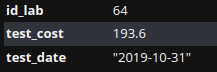
\includegraphics[width=0.3\linewidth]{Imagens/Neo4j/lab_screening.png}
    \caption{Exemplo de um nodo testes médicos}
    \label{fig:nodo_testes_medicos}
\end{figure}

\section{Hospitalização}\label{secHospitalizacao}
\begin{figure}[H]
    \centering
    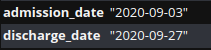
\includegraphics[width=0.3\linewidth]{Imagens/Neo4j/hospitalization.png}
    \caption{Exemplo de um nodo hospitalização}
    \label{fig:nodo_hospitalizacao}
\end{figure}

\section{Quarto}\label{secQuarto}
\begin{figure}[H]
    \centering
    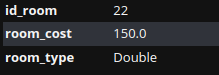
\includegraphics[width=0.3\linewidth]{Imagens/Neo4j/room.png}
    \caption{Exemplo de um nodo quarto}
    \label{fig:nodo_quarto}
\end{figure}

\section{Contador}\label{secContador}
\begin{figure}[H]
    \centering
    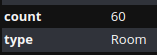
\includegraphics[width=0.3\linewidth]{Imagens/Neo4j/counter.png}
    \caption{Exemplo de um nodo contador}
    \label{fig:nodo_contador}
\end{figure}


%\end{appendices}
